\documentclass[12pt,a4paper]{article}
\usepackage{fontenc}[T1]
\usepackage[english]{babel}
\usepackage[utf8]{inputenc}
\usepackage{algorithm}
\usepackage[noend]{algpseudocode}
\usepackage{amsfonts}
\usepackage{amsmath, array}
\usepackage{amsthm}
\usepackage{vmargin}
\usepackage{multicol}
\usepackage{graphicx}
\usepackage{caption}
\usepackage{subcaption}
\usepackage{enumerate}
\usepackage{mathtools}
\usepackage{tikz}
\definecolor{violet}{cmyk}{0.79,0.88,0,0}
\long\def\symbolfootnote[#1]#2{\begingroup%
\def\thefootnote{\fnsymbol{footnote}}\footnote[#1]{#2}\endgroup}

\tikzstyle{vertex}=[draw,circle,text=violet,minimum width=20pt]
\setmargrb{19.0mm}{12.0mm}{19.0mm}{12.0mm}%{left}{up}{right}{down}

\DeclarePairedDelimiter\ceil{\lceil}{\rceil}
\DeclarePairedDelimiter\floor{\lfloor}{\rfloor}
\providecommand{\myceil}[1]{\left \lceil #1 \right \rceil }
\providecommand{\myfloor}[1]{\left \lfloor #1 \right \rfloor }

\newtheorem{theorem}{Theorem}
\newtheorem{corollary}{Corollary}
\newtheorem{lemma}{Lemma}
\newtheorem{definition}{Definition}
\newtheorem*{remark}{Remark}
\newcommand{\pa}{\mathtt{a}}
\newcommand{\pb}{\mathtt{b}}
\newcommand{\pl}{\mathtt{l}}

\title{Exact Bounds for Coin Weighing \\ by Pairwise Comparisons}
\author{Te-Sheng Tan\footnote{Tan and Wu are co-first authors and main contributors of this work.} \and Dai-Yang Wu$^\fnsymbol{footnote}$ \and Wing-Kai Hon}
\date{}
\begin{document}
\maketitle
\section{Introduction}

There is a classic puzzle about counterfeit coin problem: a man has 12 coins among which there has a counterfeit coin, which can only be told apart by its weight. How can one tell in not more than three weighings and determine which one is a counterfeit coin [1].  \\


The problem was so popular that have many other variants[2], for example, the weight of counterfeit coin is heavy or light are known; given an extra coin known to be real; or even answer the question by using a spring balance i.e. a weighing device that will return the exact weight. Halbeisen[3] generize this problem when we are allowed to use more than 1 balances and consider more than one counterfeit coin.  \\



Here we extend this question by a new direction: Now we have $\pa$ real coins and $\pb$ counterfeit coins ($ \pa, \pb > 0$). The real coins are all the same weight and also the counterfeit coins, but two  type are different weight. Each time we compare only two coins have the same weight or not. In this case, assume $\pa$, $\pb$ are known. We want to study the smallest number of comparison that we can guarantee to find a real coin and a fake one (don't need to know which one is real). \\

We compare only two coins in each time which can transfer to a new circumstances: 
there is an engine broken because of burned wire, and we need to find a pair of new electric wires to fix it, but all the wire are mass up, we only know that we have $\pa$ positive wires and $\pb$ negative wires in the beginning, each time we can choose 2 of them to connect to the engine and check if they are the same Electrical polarity (not work) or not (work). The object is minimize the worst case of testing times that we can fix the engine.  \\


\section{An Equivalence Graph Problem}


\subsection*{Idea}
We can present a set of comparisons as a graph. Vertice are the coins, edges are the comparisons.

Consider a graph ${\cal G}(\pa,\pb)$ contains two part, one is $K_\pa$, another is $K_\pb$, then we want to find a graph $g(\pa,\pb)$ (number of vertices $\leq \pa+\pb$), and $g(\pa,\pb)$ is not a subgraph of ${\cal G}(\pa,\pb)$. 
Let $t =$ number of edges of $g(\pa,\pb)$, then through these $t$ comparisons, at least one of them is unbalanced.

\begin{proof}

Prove by contradiction.

Denote the real coins as '+' and the fake ones as '-'. 

We compare edges of g(a,b). If we found all balance in these t comparison, we can assign a '+'s and b '-'s into g(a,b), then g(a,b) is the subgraph of ${\cal G}(\pa,\pb)$.
\end{proof}

Intuitively, if finding unbalance in a comparison, the game ends. But sometimes we can point a pair is unbalance after k comparisons(k is the answer) before the unbalance appears. The following shows $k_{min}=t_{min}-1$, which means the answer for Problem 4 is $t_{min}-1$

\begin{lemma}
$t_{min} = k_{min}+1 $
\end{lemma}

\begin{proof}
We divide the proof of the equation into two inequations

If we could point out a pair $e$ is unbalanced through the optimal graph $F$(with $k_{min}$ comparisons).
Consider a graph with these $k_{min}$ edges + $e$ which is not a subgraph of ${\cal G}(\pa,\pb)$
\[t_{min}\leq k_{min}+1\]

For a optimal graph $E$(with $t_{min}$ edges) which is not a subgraph of ${\cal G}(\pa,\pb)$. Let $E'$ = ($E$ remove an arbitrary edge $e$), then through $E'$

If $E'$ has unbalance comparison, we conclude the one is unbalanced, otherwise we could conclude $e$ is unbalanced.

Either case shows $E'$ is enough to end the game.
\[k_{min} \leq t_{min}-1\]

From the above inequations, the lemma holds.

\end{proof}

\subsection*{Goal}
We want to find a graph $g(\pa,\pb)$ that has minimum edges and $g(\pa,\pb)$ is not a subgraph of ${\cal G}(\pa,\pb)$. Through testing $g(\pa,\pb)-$an arbitrary edge $e$, we can point out a pair is unbalanced and it's optimal.

If comparing the edges of a graph results in at least one unbalanced edge in any condition.
We say this graph is a testing solution, feasible. Otherwise it's infeasible.

A testing solution(or a solution) is presented by graph.

\begin{definition}
An optimal testing solution(denoted by $OTS$) is a solution with minimum number of edges(comparisons).
\end{definition}

An $OTS$ can presented by an integer partition as well, which is covered in Section 3.

\begin{definition}
$\tau(\pa,\pb)$ is the number of edges of $OTS(\pa,\pb)$
\end{definition}

For example, $\tau(1,2)=2$, since testing a pair may result in balanced. On the other hand, testing two non-duplicate pair, one of them must results in unbalanced.

In this case, testing a pair is enough to point out a real coin and a fake one. 

Denote the coins we test as $coin_a$ $coin_b$ , the coin we didn't test as $coin_c$
If $coin_a$ and $coin_b$ is not balanced, then point out $coin_a$ and $coin_b$. Otherwise, point out $coin_a$ and $coin_c$
\section{Integer Partition}

\noindent
To find $g(\pa,\pb)$ with minimal number of edges, it's obvious that $g(\pa ,\pb)$ should not form a cycle

\begin{proof} 
if $g(\pa,\pb)$ form a cycle, remove an edge, the number of vertices each component remains same, whether $g'(\pa,\pb)$ is the subgraph of ${\cal G}(\pa,\pb)$ is equivalent to whether $g(\pa,\pb)$ is the subgraph of ${\cal G}(\pa,\pb)$
\end{proof}

\begin{definition}
We define a multiset avoids $x$ if its subset-sums has no $x$, a partition avoids if its parts avoids $x$
\end{definition}

\begin{theorem}

the problem would be transformed to find a partition of $\pa+\pb$ with  maximal number of parts that avoids $\pa$

\end{theorem}

\begin{proof} 
Let $t =$ number of edge of $g(\pa,\pb)$

$n$ as number of componets in $g(\pa,\pb)$

$M$ as the set of components

$m$ as the set of number of vertices

$m_i$  as number of vertices of $i$th component

since $g(a,b)$ doesn't contain any cycle, $t = \pa+\pb - n$, to find minimal t is equivalent to find maximal n such that $g(\pa,\pb)$ is not the subgraph of ${\cal G}(\pa,\pb)$

if $g(\pa,\pb)$ is the subgraph of ${\cal G}(\pa,\pb)$, 
since each component is conected, each one is either in $K_a$ or $K_b$, there exist a subset of M in $K_a$ the number of vertices of M = a
,e.g there exist a subset of m is equal to $a$

if $g(\pa,\pb)$ is not the subgraph ${\cal G}(\pa,\pb)$, there must not a subset of m is equal to $a$, since if there subset of m is equal to $a$ let these componets in $K_a$ and others in $K_b$, then $g(\pa,\pb)$ is the subgraph ${\cal G}(\pa,\pb)$ thus raise contradiction


the sum of $m$ is $\pa+\pb$, so the theorem holds

\end{proof}

\begin{definition}
$\rho(\pa,\pb)$ is the maximal number of parts of $\pa+\pb$ avoids $\pa$

$d$ is the smallest non-factor of $\pa$
\end{definition}

\begin{remark}
$\tau(\pa,\pb)=\pa+\pb-\rho(\pa,\pb)$
\end{remark}

\begin{theorem}
Optimal partition for $\pa=2$

\[
 \rho(2,\pb) =
   \begin{cases}
     1+\frac{\pb}{3}   &\mbox{if }\pb\equiv0\\
     1+\frac{\pb-1}{3} &\mbox{if }\pb\equiv1\\
     1+\frac{\pb+1}{3} &\mbox{if }\pb\equiv2
   \end{cases}
   \pmod{3}
\]
\end{theorem}

\begin{proof}
	since there is no $a$ in subset sums of the partition $P$, there is at most one '$1$' and no '$2$' in $P$, $|P|\leq \floor{\frac{\pb+2}{3}}$

	for $\pb\equiv0\pmod{3}$, there exist an optimal partition $P=\{1,4,3,...\}$('...' are '$3$'s) that reaches optimal bound and avoids $\pa$

	for $\pb\equiv1\pmod{3}$, there exist an optimal partition $P=\{1,5,3,...\}$('...' are '$3$'s) that reaches optimal bound and avoids $\pa$

	for $\pb\equiv2\pmod{3}$, there exist an optimal partition $P=\{1,3,3,...\}$('...' are '$3$'s) that reaches optimal bound and avoids $\pa$

\end{proof}


\subsection{Exact Algorithm}

\begin{algorithmic}
  \STATE{$R= \{\pa+\pb\}$}
  \FOR{\textbf{each} partition $P$ of the number $\pa+\pb$}
    \IF{$P$ avoids $\pa$ \AND{$|P|>|R|$}} \STATE{$R=P$}
    \ENDIF
  \ENDFOR
  \STATE{output $R$}
\end{algorithmic}
check P's avoidence by Dynamic-Programming as solving discrete knapsack problem, keep avoidence vector when enumerating.

Time Complexity: $O(\pa\frac{exp(\sqrt{\frac{2(\pa+\pb))}{3} } )}{\pa+\pb})$

\subsection{Results}


\section{Futher Speedup}

\begin{lemma}
$\rho(a,b)$ has lower-bound $\ceil{\frac{b}{d}}$
\end{lemma} 

\begin{proof}
To proof a lower-bound, we show a case whose number of partitions=$\ceil{\frac{b}{d}}$

The case is trivial, divide $a+b$ into $\ceil{\frac{b}{d}}-1$ instances of $d$ and a $a+b-d\ceil{\frac{b}{d}}-1$ (denoted by $s$)

Prove the case avoids $\pa$ by contradiction

If the subset contains $s$ since $s>a$ $\implies$ contradiction

If the subset doesn't contains $s$, it contains only several $d$, but since $d\not| a$ $\implies$ contradiction
\end{proof}

\begin{lemma}
If a multiset $S$ avoids $a$ and composed only by factors of $a$, 

$|S|<a$
\end{lemma}

\begin{proof}

We shall prove this by contradiction

We denote the number of $i$ in $S$ as $X_i$, that is, we have $X_i$ '$i$'(s) in $S$

, the first $k$ elements of $S$ as $S_k$. $S_0$ is the empty set.

We define set $U(s)$ for a multiset $s$ as subset-sums$\leq a$ of $s$. For example, $\pa=5$, $U({1,3,3})=ignore_{>5}(\{ 0,1,3,4,6,7\})=\{ 0,1,3,4\}$

% \begin{remark}
Note that for any $s$, $U(s)$ always include zero.
% \end{remark}

We divide the proof into two sections.

1. $\forall k, |U(P_{k+1})|>|U(P_k)| $ 

Denote $U(P_{k+1})$ as $u'$ and $U(P_k)$ as $u$.

Prove this by contradiction, if $|u'|=|u|$ for some $k$, let $w$ is the k+1th element of $S$,then 
Since $u\subseteq u'$, $u=u'$

$\forall i\geq w, i \in u \implies i+w\in u' \implies i+w\in u$

Since U always include 0, $0\in u \implies tw\in u \forall t$

$w$ is a factor of $\pa$, thus $w\in u$, contradicts $S$ avoids $\pa$

2. We discover $U(S_0)$ to $U(S_{|S|})$, since $U(S_0)=\{0\}$, each time
$U$ at least a new element. If $|S|\geq \pa$, then $U(S)$
must be $\{0,1,...,\pa\}$, contradicts $S$ avoids $\pa$


\end{proof}

\begin{theorem} 
$\forall \pb>d(d+1)(\pa-1)  + (\pa - (\pa\mod d)$, an optimal partition contains at least $\floor{{\frac{\pa}{d}}}$ instances of $d$
\end{theorem}

\begin{proof} 
    Let $S$ is a partition of $\pa+\pb$ avoids $\pa$,   $X_i$ is the number of times $i$ appears in $S$  and  $X = \sum_i{X_i}$  \\  

    Assume $X_d<\lfloor{\frac{\pa}{d}} \rfloor $, \\

    Then 
    \[
    X=\sum_{i<d}{X_i}+X_d+\sum_{i>d}{X_i}
    \]
    Since $\sum_i{X_i\times i}=\pa+\pb$, to maximize $X$, we use as much small number as possible. Hence

    \begin{align*}
    X&\leq \pa-1+ \floor{\frac{\pa}{d}}   +\floor{{\frac{\pb-(\pa - (\pa\mod d))}{d+1}}}\\
     &\leq \pa-1+ \frac{\pa}{d}   +{\frac{\pb-(\pa - (\pa\mod d))}{d+1}}
    \end{align*}
    
    $\forall \pb>d(d+1)(\pa-1) + (\pa - (\pa\mod d)), \\
    X<\pa+\floor{\frac{\pa}{d}} + \pa d -d \leq \ceil{\frac{\pb}{d}}$.    contradicts lemma 4.1

    Hence  S is not optimal
\end{proof}

\begin{theorem}
	$\forall \pb>d(d+1)(\pa-1)  + (\pa - (\pa\mod d)$, $\rho(\pa,\pb+d)=\rho(\pa,\pb)+1$
\end{theorem}

\begin{proof}
    $S$ is a optimal partition of a+b avoids $a$ ($b>d(d+1)(a-1)  + (a - (a\mod d)$)
    
    $S'=S+$'d' is a partition of a+b+d 

    We divide the proof into avoidance part and optimal part

    {\bf(Avoidance)}
    Prove this by contradiction

    If $S'$ has subset-sum $\pa$, $S$ must has subset-sum $\pa$ or $\pa-d$. The former is not possible from definition. 

    If the later happens, $S$ has subset-sum $\pa$ since it has at least $\floor{{\frac{a}{d}}}$ instances of 'd', and $\pa-d$ couldn't has all of them.
    Also contradict definition.

    $S'$ avoids $\pa$.

    {\bf(Optimal)}
        prove by contradiction

        If $S'$ is not optimal there exist an optimal partition $P'$ that $|P'|>|S'|$ and has no subset-sum=$a$

        $P'$ has at least one $d$, let $P=P'-d(sum(P)=sum(S))$ then $P$ has no subset-sum=$a$ and $|P|=|P'|-1>|S'|-1=|S|$, which contradicts $S$ is optimal.

        $S'$ is optimal.

    Thus the theorem holds.
\end{proof}

\begin{corollary}
for a constant $\pa$, $\rho(\pa,\pb)$ forms cycle of length $d$ if $\pb$ is sufficiently large
\end{corollary}

\subsection{Algorithm using cycle property}

let $K=\pa+\pb-kd>d(d+1)a$ (choose maximal $k$, e.g. minimal $K$)

\begin{algorithmic}
  \STATE{$R= \{\pa+\pb\}$}
  \FOR{\textbf{each} partition $P$ of the number K which avoids $\pa$}
    \IF{$|P|>|R|$} \STATE{$R=P$}
    \ENDIF
  \ENDFOR
  \STATE{output $R$+k instances of 'd'}
\end{algorithmic}
check P's avoidence by Dynamic-Programming as solving discrete knapsack problem, keep avoidence vector when enumerating.

Time Complexity:

Denote the number of partitions of $n$ as $p(n)$

Denote the number of partitions avoids $a$ of $n$ as $p_{aoivds\ a}(n)$

\[
O(k+a\times p_{aoivds\ \pa}(K))\\
= O(\pa\times p(K))\\
= O(\pa\frac{exp(\sqrt{\frac{2(1+d(d+1)(\pa-1)+\pa)}{3} } )}{1+d(d+1)(\pa-1)+\pa})
= O(\frac{exp(\sqrt{\frac{2(1+d(d+1)(\pa-1)+\pa)}{3} } )}{d^2})
\]
\section{extended problem}
We shall discuss several problems simular to the foolproof problem in section 1. These are called inference problems. For convenience, we assume fake coins are minor in the whole coins.(e.g. ($\pa\leq \pb $)
In the same way in Section 2, we present a scheme as a graph. There are four inference problems: infering a fake coin,a real coin, real-fake pair, a fake coin and a real coin. We $-$, $+$, $\pm$, $+-$ superscription to denote them seperately.

\subsection*{Infering a real-fake pair}
{
\setlength{\leftskip}{1cm}
\setlength{\rightskip}{1cm}
There are $\pa$ fake coins and $\pb$ real coins ($\pa, \pb > 0$). The real coins are all the same weight and also the counterfeit coins, but two  types are different weight. Each time we compare only two coins have the same weight or not. In this case, assume $\pa$, $\pb$ are known.
Find the smallest number of comparison that we can infer a pair is real-fake. In this problem, we don't need to know which one is fake.\\

}
\begin{definition}
If a scheme could infer a real-fake coin. We say this graph is a inferable$^\pm$ scheme for fake ($\IS^\pm$). Otherwise it's not inferable$^\pm$.

Optimal inferable scheme for fake ($\OIS^\pm$) is $\IS^\pm$ with minimum number of comparison.
Deonte the number of edges of $\OIS^\pm$ by $\tau^\pm(\pa,\pb)$.
\end{definition}

Note that in the foolproof problem. We can infer the pair on the scale which is unbalanced. But sometimes before the unbalance appears, we can infer a pair is real-fake. The following shows the answer is $\tau(\pa,\pb)-1$.

\begin{lemma}
$\OIS^\pm= \text{removing an arbitrary edge}$. That is, $\tau^\pm(a,b)=\tau(a,b)-1$
\end{lemma}

\begin{proof}
We divide the proof of the equation into two inequations. For conciseness, we denote $\tau(a,b)-1$ by $\tau$ and the answer of this problem as $\tau^\pm$.

For a optimal foolproof scheme $G$(with $\tau$ edges). Let $G'$ = ($G$ remove an arbitrary edge $e$), then through $F'$.
If $G'$ has unbalance comparison, we conclude the one is unbalanced, otherwise we could conclude $e$ is unbalanced.
Either case shows $G'$ is sufficient to infer a real-fake pair.
\[\tau^\pm \leq \tau-1\]

If we could infer a pair $e$ is real-fake through the optimal scheme $F$(with $\tau^\pm$ comparisons).
Then the graph $F$ + $e$ is foolproof.
\[\tau\leq \tau^\pm+1\]

From the above inequations, the lemma holds.

\end{proof}
\subsection*{Two conditions of a testing scheme}

When testing a testing scheme, there are two conditions.

\textbf{Condition 1.} there is an unbalanced edges

\textbf{Condition 2.} they are all balanced

For infering a $\pm$, we must ganrantee both conditions work. For Condition 1, we would simplily infer the unbalanced edges. For Condition 2, we would infer the edge must be unbalanced because adding this edge would form a foolproof scheme.
For the following inference problems($-$,$+$,$+-$), we shall use the same logic. 

\subsection*{Infering a fake coin}
{
\setlength{\leftskip}{1cm}
\setlength{\rightskip}{1cm}
\noindent 
There are $\pa$ fake coins and $\pb$ real coins ($\pa, \pb > 0$). The real coins are all the same weight and also the counterfeit coins, but two  types are different weight. Each time we compare only two coins have the same weight or not. In this case, assume $\pa$, $\pb$ are known.
Find the smallest number of comparison that we can infer a coin is fake.\\

}


\begin{definition}
Same as previous problem, we define $\IS^-$, $\OIS^-$ and $\tau^-(a,b)$.
\end{definition}

Note that $\OFS(a,b)$ could find a real and a fake coin. Thus $\tau(\pa,\pb)$ is an upper bound of $\tau^-(\pa,\pb)$.
A $\IS^-(\pa,\pb)$ better than $\OFS(\pa,\pb)$ must use another strategy, which is, though all comparisons result in balance we could still infer a `$-$'.\\

Before solving $\IS^-$, we observe how a inferable$^-$ scheme works.

For a testing scheme, there are two conditions

If \textbf{Condition 1.} happens then we immediate infer the fake coin from the unbalanced.
If \textbf{Condition 2.} happens, we must claim a fake coin, and this coin couldn't be a real one in any condition, otherwise this inference is wrong.\\

We present an optimal inferable$^-$ scheme as a integer partition for an example. Let (a,b)=(2,6), 
this scheme is [3,3,`1',1] .If \textbf{Condition 2}, we infer the `1' is the fake coin. To explain more, we introduce the following lemma.

\begin{lemma}\label{lma:inferable}
If \textbf{Condition 2}, the scheme is inferable for a fake coin $c_1$ if and only if removing $c_1$'s part, the remaining parts avoids $\pa$. Physically, $c_1$ must not be a real coin with \textbf{Condition 2}.
\end{lemma}

To find a inferable$^-$ better than $\OFS$ must solve \textbf{Condition 2}.
Denote the part of the fake coin to be infered as $i(i\leq\pa)$. 
Beyound the remainning $\pa+\pb-i$ parts, 
(1)they must avoid $\pa$, since if there's a subset sum $\pa$, assign the subset `$+$', this claim is wrong
(2)they must contain $\pa-i$ or equivalently contain $\pb$, since there must exist a condition such that the coin is fake and \textbf{Condition 2}.


\begin{definition}
For convenience, we define $Q(n,a,b)$ as the number of edges that avoids $\pa$ but contains $\pb$ 
\end{definition}

Note that $Q(n,a,b)\geq\tau(a,n-a)$\\

For \textbf{Condition 2.}, $1\leq i\leq\pa$ for $\IS^-$, thus we get the following lemma.

\begin{lemma}
$\tau^-(\pa,\pb)=min\{\tau(\pa,\pb), \{i-1+Q(\pa+\pb-i,\pa,\pb) | 1\leq i\leq\pa\} \}$
\end{lemma}

We are ready to solve $\OIS^-$ now.

\begin{theorem}
$\OIS^-(\pa,\pb)=optimal\{\OFS(a,b), \{\text{a tree of i-1 nodes and }\OFS(a,b-i) |1\leq i\leq a\}\}$

$\tau^-(\pa,\pb)=min\{\tau(\pa,\pb), \{i-1+\tau(\pa,\pb-i) | 1\leq i\leq\pa\} \}$
\end{theorem}

\begin{proof}
We divide the proof into inferable$^-$ part and optimal part.

\noindent{\bf (inferable$^-$ Part:)}

For $OFS(a,b)$ could infer a fake coin because only \textbf{Condition 1.} happens.
For $\{\text{a tree of i nodes and }OFS(a,b-i) |1\leq i\leq a\}\}$, if \textbf{Condition 2.}, we infer one coin of the i-node tree as fake coin.

\noindent{\bf (Optimal Part:)}
from lemma 5.2
\begin{align*}
\tau^-(a,b)&=min\{\tau(a,b),\{i-1+Q(a+b-i,a,b) | 1\leq i\leq a\} \}\\
&\geq min\{\tau(a,b), \{i-1+\tau(a,b-i) | 1\leq i\leq a\} \}
\end{align*}

is a optimal lower bound.

And $optimal\{OFS(a,b), \{\text{a tree of i nodes and }OFS(a,b-i) |1\leq i\leq a\}\}$ reaches this lower bound.

\end{proof}

\subsection*{Infering a real coin}

{
\setlength{\leftskip}{1cm}
\setlength{\rightskip}{1cm}
\noindent 
There are $\pa$ fake coins and $\pb$ real coins ($\pa, \pb > 0$). The real coins are all the same weight and also the counterfeit coins, but two  types are different weight. Each time we compare only two coins have the same weight or not. In this case, assume $\pa$, $\pb$ are known.
Find the smallest number of comparison that we can infer a coin is real.\\

}

\begin{definition}
Same as previous problem, we define $\IS^+$, $\OIS^+$ and $\tau^+(a,b)$.
\end{definition}

$\OIS^+$ is trivial.
That is, comparing $\pa$ coins in a group. 

\begin{theorem}
$\OIS^+(\pa,\pb)=\text{a tree of }\pa+1\text{ nodes}$
\end{theorem}
\begin{proof}
We divide the proof into inferable$^+$ part and optimal part.

\noindent{\bf (Inferable$^+$ Part:)}

we omit this part since it's same as previous theorem.

\noindent{\bf (Optimal Part:)}
\begin{align*}
\tau^+(a,b)&=min\{\tau(a,b), \{i-1+Q(a+b-i,b,a) | 1\leq i\leq b\} \}&\\
&\geq min\{\tau(a,b), \{i-1+\tau(a-i,b) | 1\leq i\leq b\} \} &\text{by Theorem 2.2.}\\
&\geq min\{\floor{\frac{a+b}{2}}, i-1+\frac{a-i+b}{2}\}&\\
&\geq min\{a, a\}=a &
\end{align*}

is a optimal lower bound.

$\text{a tree of }\pa+1\text{ nodes}$ reaches optimal lower bound.
\end{proof}

\subsection*{Infering a real coin and a fake coin}

{
\setlength{\leftskip}{1cm}
\setlength{\rightskip}{1cm}
\noindent 
There are $\pa$ fake coins and $\pb$ real coins ($\pa, \pb > 0$). The real coins are all the same weight and also the counterfeit coins, but two  types are different weight. Each time we compare only two coins have the same weight or not. In this case, assume $\pa$, $\pb$ are known.
Find the smallest number of comparison that we can infer a coin is real and another coin is fake.(e.g. a real-fake pair that we know which one is fake)\\

}
\begin{definition}
Same as previous problem, we define $\IS^{+-}$, $\OIS^{+-}$ and $\tau^{+-}(a,b)$.
\end{definition}

This problem seems the same as the foolproof problem, but not exactly. The difference is whether the real-fake pair need to be compared on the scale. For most cases, OFS is optimal for this problem but not all cases. That is, the answer is $\tau$. Consider $(\pa,\pb)=(3,8)$, there's a OFS, [2, 2, 2, 5]. An edge removed, the scheme [2, 2, 2, `4', `1'] is not only inferable$^\pm$ but also $^+-$(`4' and `1').(see explaination in Figure) In this case, the answer is $\tau-1$.
\begin{figure}[!htb]
   \centering
    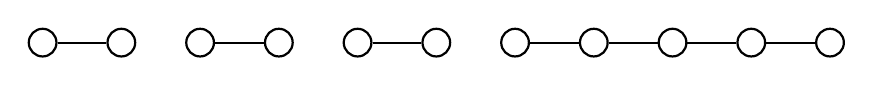
\begin{tikzpicture}[auto, thick]
\tikzstyle{vertex}=[draw,circle,text=violet,minimum width=10pt]
  \foreach \place/\name in {{(0,0)/a},
                            {(1,0)/b},
                            {(2,0)/c},
                            {(3,0)/d},
                            {(4,0)/e},
                            {(5,0)/f},
                            {(6,0)/g},
                            {(7,0)/h},
                            {(8,0)/i},
                            {(9,0)/j},
                            {(10,0)/k}}
    \node[vertex] (\name) at \place {};
  \foreach \source/\dest in {a/b,c/d,e/f,g/h,h/i,i/j,j/k}
      \path (\source) edge (\dest);
\end{tikzpicture} \vspace*{2.5ex}
    \caption{A foolproof scheme for $(\pa,\pb)=(3,8)$}
\end{figure}

\begin{figure}[!htb]
   \centering
    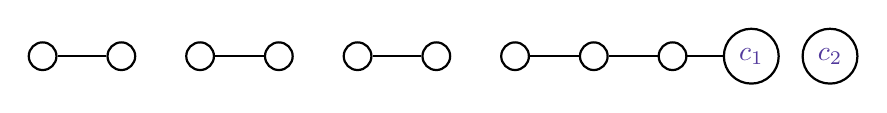
\begin{tikzpicture}[auto, thick]
\tikzstyle{vertex}=[draw,circle,text=violet,minimum width=10pt]
  \foreach \place/\name in {{(0,0)/a},
                            {(1,0)/b},
                            {(2,0)/c},
                            {(3,0)/d},
                            {(4,0)/e},
                            {(5,0)/f},
                            {(6,0)/g},
                            {(7,0)/h},
                            {(8,0)/i}}
    \node[vertex] (\name) at \place {};
  \node[vertex] (j) at (9,0) {$c_1$};
  \node[vertex] (k) at (10,0) {$c_2$};
  \foreach \source/\dest in {a/b,c/d,e/f,g/h,h/i,i/j}
      \path (\source) edge (\dest);
\end{tikzpicture} \vspace*{2.5ex}
    \caption{An $\IS^{+-}$ for $(\pa,\pb)=(3,8)$. If there is an unbalance edge, we infer the fake and real coin of the pair. If edges are all balance, we can infer the coin $c_1$ is real and the coin $c_2$ is fake.}
\end{figure}

Before discussing how to find an $\IS^{+-}$, we observe the range of $\tau^{+-}(a,b)$. Since $\tau(\pa,\pb)$ is sufficient to infer a fake coin and a real coin. 

\[
\tau^{+-} \leq \tau
\]

Through we cound infer a fake coin and a real coin, add this edge into the $\OIS^{+-}$, it's foolproof.

\[
\tau \leq \tau^{+-}+1
\]

Combine the inequations

\[
\tau-1 \leq \tau^{+-} \leq \tau
\]


Before solving $\IS^{+-}$, we observe how this works.

If \textbf{Condition 1.} happens then the solution works.
If \textbf{Condition 2.} happens, we infer a fake coin and a real coin. This pair is not in the $\IS^{+-}$. Adding this pair(edge) into the $\IS^{+-}$, the new graph is foolproof.

\begin{lemma}
Any inferable$^{+-}$ scheme is either a foolproof scheme or a foolproof scheme with an edge removed.
\end{lemma}

\begin{theorem}
Any optimal inferable$^{+-}$ scheme is either a optimal foolproof scheme or an optimal foolproof scheme with an edge removed.
\end{theorem}

Unlike infering a real-fake pair, removing an arbitrary edge from a $\OFS$ may not work.
We enumerate the edge removed for each $\OFS$ then check whether it's inferable$^{+-}$. 
Checking a scheme's inferability$^{+-}$ is similar to checking its inferability$^+$. Condition 1 is simple and the scheme to ganrantee Condition 2 don't happen is $\FS$. We shall focus on Condition 2. If Condition 2 happen can we infer a $+-$? To explain more, we return to the case Figure 4, the reason Figure 4 works is from lemma \ref{lma:inferable}. Because removing $c_1$'s component, the multiset [2,2,2,1] avoids $\pb$
\section{Open questions}
\subsection{Cycle happens earlier}
    As in theorem 4.3 and 4.4, we proved $\rho(\pa,\pb)$ would be in cycle for $\pb>d(d+1)(\pa-1)+(\pa-(\pa\mod d)$. But observing $\rho$table in Results 3.2, $\rho$ seems to get in cycle earlier. After computer comfirmation, we got results bellow.
    
\begin{tabular}{lll}
 $\pa$  & $\pb$: $\rho(\pa,\pb)$ start to cycle by theorem & $\pb$: $\rho(\pa,\pb)$ start to cycle by computer comfirmation \\
\hline
 1  & 1                                     & 1                                                   \\
 2  & 13                                    & 1                                                   \\
 3  & 15                                    & 5                                                   \\
 4  & 40                                    & 10                                                  \\
 5  & 29                                    & 9                                                   \\
 6  & 105                                   & 29                                                  \\
 7  & 43                                    & 13                                                  \\
 8  & 91                                    & 22                                                  \\
 9  & 57                                    & 17                                                  \\
 10 & 118                                   & 28                                                  \\
\hline
\end{tabular}

    Since the algorithm cost exponential time, we could only comfirm this in small case.
    
    But if it get in cycle earlier in general case, we can use a better(smaller) $K$ algorithm 4.1 and run faster.
\subsection{Avoidance integer partition}
    As in algorithm 3.1,4.1, to find an optimal solution require enumerating partitions of $\pa+\pb$ avoiding $\pa$. In the algorithms, we enumerating all partitions of $\pa+\pb$ and check if it avoids $\pa$. So the time complexity is analyzed as the (number of partitions) times checking avoidance. If exist a way to enumerate avoidance and bound it tighter, the time complexity would be better.
\section{Refferences}
1. Howard D. Grossman, The twelve-coin problem, Scripta Math., 11 (1945) 360-361.  \\
2. Richard K. Guy ; Richard J. Nowakowski,  Coin-Weighing Problems, The American Mathematical Monthly, Vol. 102, No. 2. (Feb., 1995), pp. 164-167.  \\
3. Lorenz Halbeisen, Norbert Hungerbfihler, The general counterfeit coin problem, Discrete Mathematics 147 (1995) 139-150.  \\


\end{document}